\section{Preliminaries for the supervised classification}

To determine whether some information about the classification might be available in the explanatory variables, a variety of graphical and statistical summaries can be used : 

\subsection{Statistical summary}
A first way to approach the problem is by showing a statistical summary of our dataset splitted in the two tumor groups.

\begin{table}[H]
\centering
\begin{tabular}{r|rr}
 & benign & malignant \\ 
  \hline
radius\_mean & 12.123 & 17.556 \\ 
  texture\_mean & 17.931 & 21.557 \\ 
  perimeter\_mean & 77.941 & 116.026 \\ 
  area\_mean & 461.304 & 989.846 \\ 
  smoothness\_mean & 0.093 & 0.103 \\ 
  compactness\_mean & 0.081 & 0.145 \\ 
  concavity\_mean & 0.047 & 0.162 \\ 
  concave.points\_mean & 0.026 & 0.088 \\ 
  symmetry\_mean & 0.175 & 0.192 \\ 
  fractal\_dimension\_mean & 0.063 & 0.062 \\ 
\end{tabular}
\end{table}
\begin{table}[H]
\centering
\begin{tabular}{r|rr}
 & benign & malignant \\ 
  \hline
radius\_mean & 3.333 & 10.444 \\ 
  texture\_mean & 14.731 & 13.264 \\ 
  perimeter\_mean & 147.290 & 487.167 \\ 
  area\_mean & 18839.566 & 140044.214 \\ 
  smoothness\_mean & 0.000 & 0.000 \\ 
  compactness\_mean & 0.001 & 0.003 \\ 
  concavity\_mean & 0.002 & 0.006 \\ 
  concave.points\_mean & 0.000 & 0.001 \\ 
  symmetry\_mean & 0.001 & 0.001 \\ 
  fractal\_dimension\_mean & 0.000 & 0.000 \\ 
\end{tabular}
\end{table}

By looking at these tables, we can get a first insight that the variables have some kind of correlation between the classification of the tumor and the explanatory variables as larger values seems to result in malignant tumors. We can jump into more graphical analysis to show in more detail the distribution of the explanatory variables relative to their classification.

\subsection{Box and density plots}
By using the box and density plots, we can easily visualize whether the two groups have different distributions for each explanatory variable by showing in a more visual way the previously computed summary values.
\\\\
As can clearly be seen in the 2 figures here under, there's a logical relationship between the tumor's size and it's classification between benign and malignant. Indeed, in the boxplots and density plots, we clearly see that the mean of each explanatory variable is distributed along smaller values for benign tumors than for malignant tumors. This relationship seems logical to us as the bigger the tumor, the more dangerous it gets. These facts, are all true except for 1 variable, \verb|fractal_dimension_mean|. All these observations results in giving us some confidence that we'll be able to classify the observations between the two groups using the majority of the explanatory variables.

\begin{figure}[H]
    \centering
    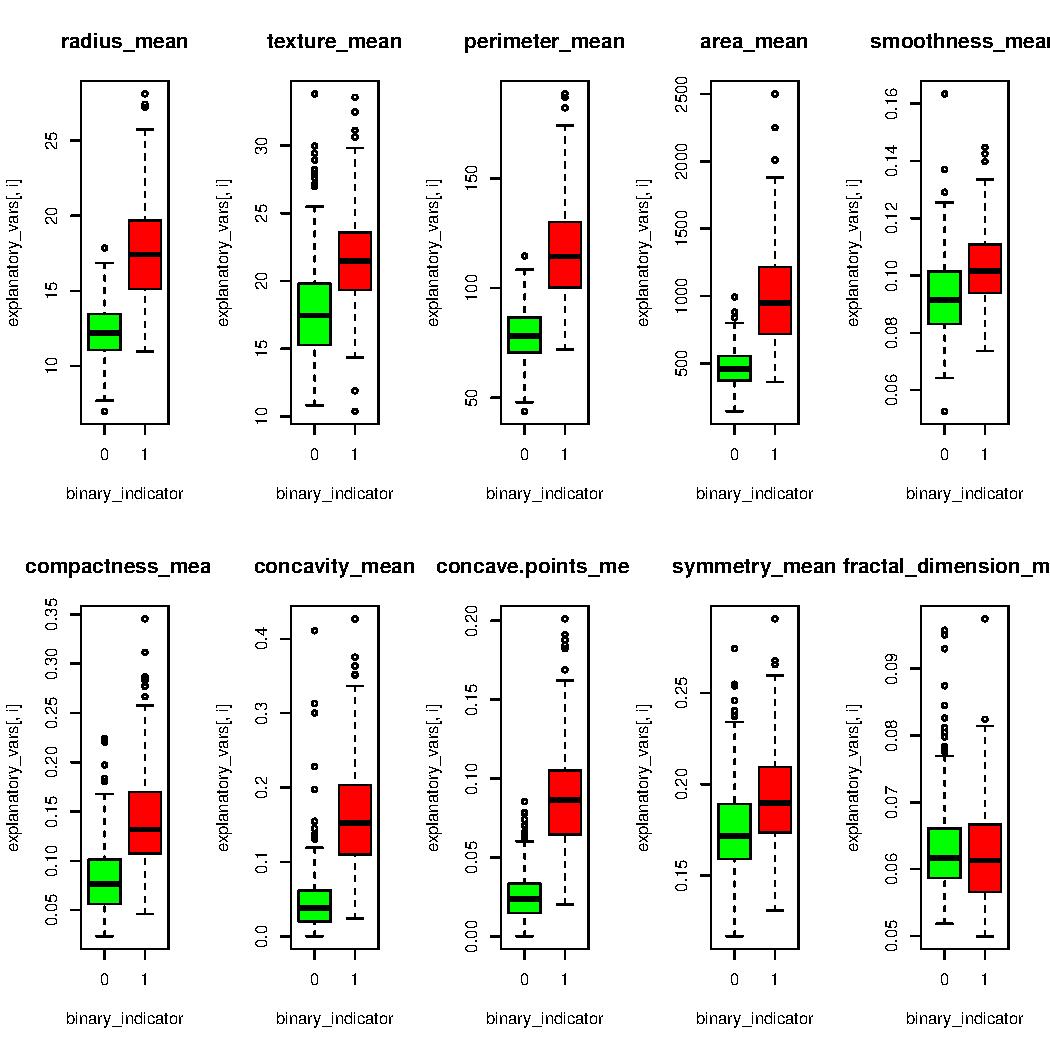
\includegraphics[width=.55\textwidth]{figs/q1_boxplot.pdf}
    \caption{Boxplot of explanatory variables separated by groups}
    \label{fig:q1_boxplot}
\end{figure}

\begin{figure}[H]
    \centering
    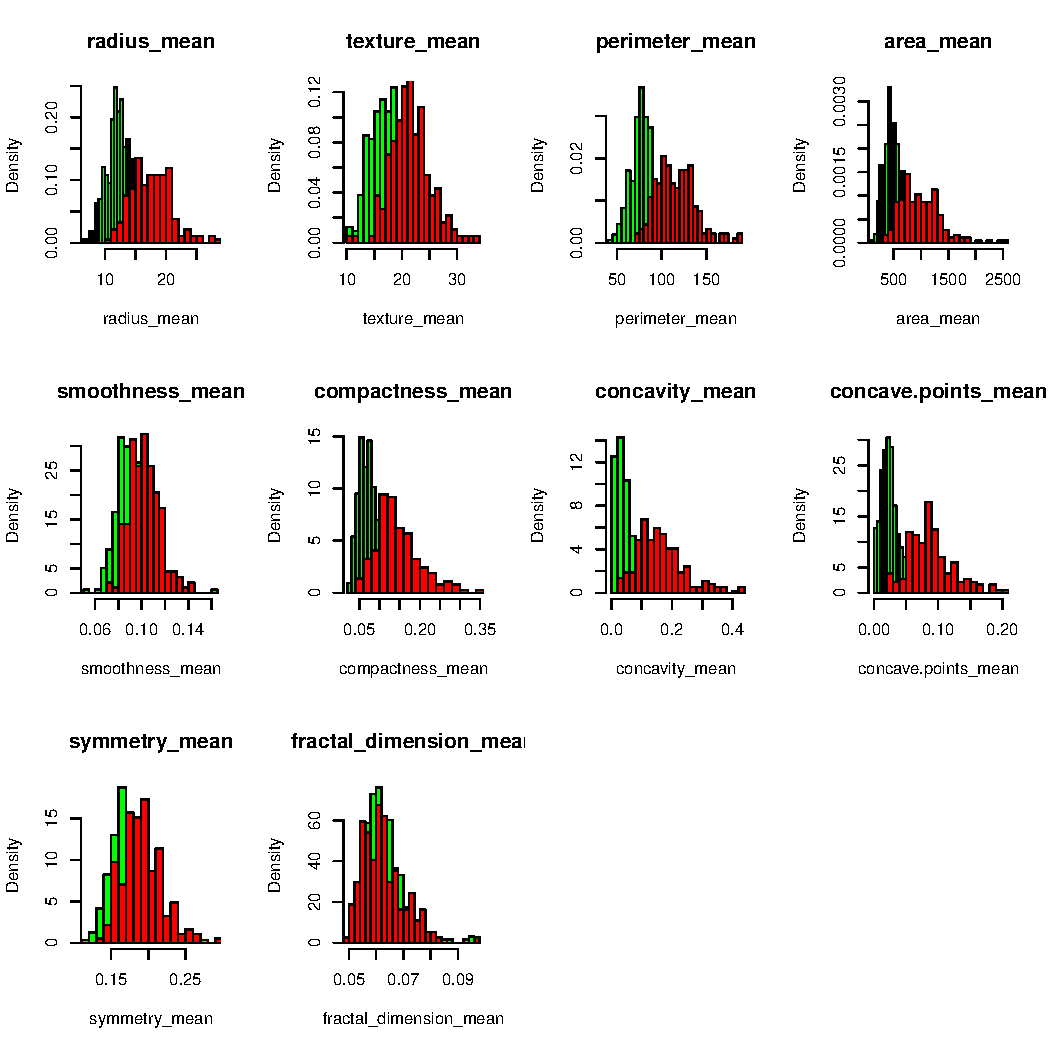
\includegraphics[width=.55\textwidth]{figs/q1_histogram.pdf}
    \caption{Density plot of explanatory variables separated by groups}
    \label{fig:q1_density}
\end{figure}

\newpage
\subsection{Correlation matrix and scatterplot}
Another method to assess if the explanatory variables can be used to classify the data between the 2 classes is a correlation matrix : 

\begin{figure}[H]
\centering
\begin{subfigure}{.5\textwidth}
  \centering
  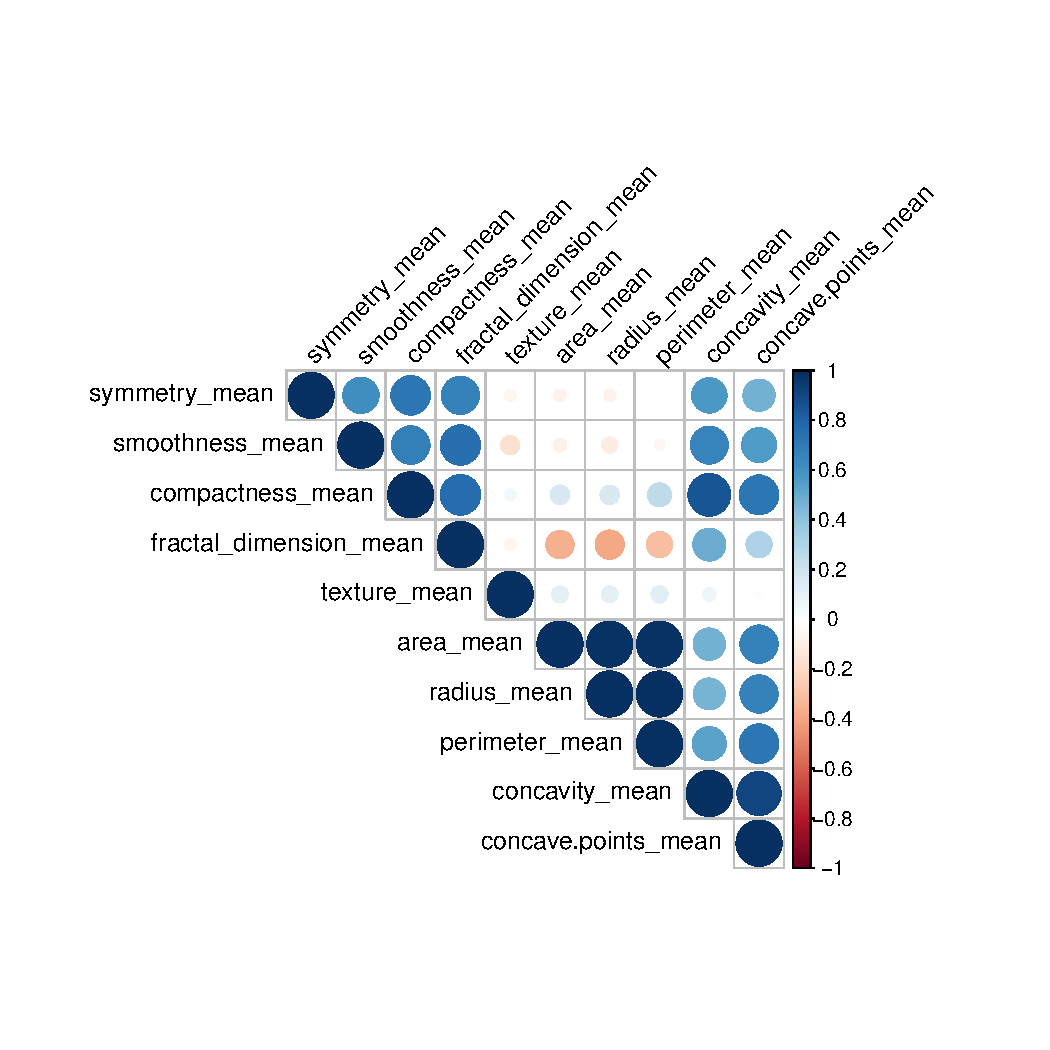
\includegraphics[width=.9\linewidth]{figs/q1_correlation_malignant.pdf}
  \caption{Malignant tumors}
\end{subfigure}%
\begin{subfigure}{.5\textwidth}
  \centering
  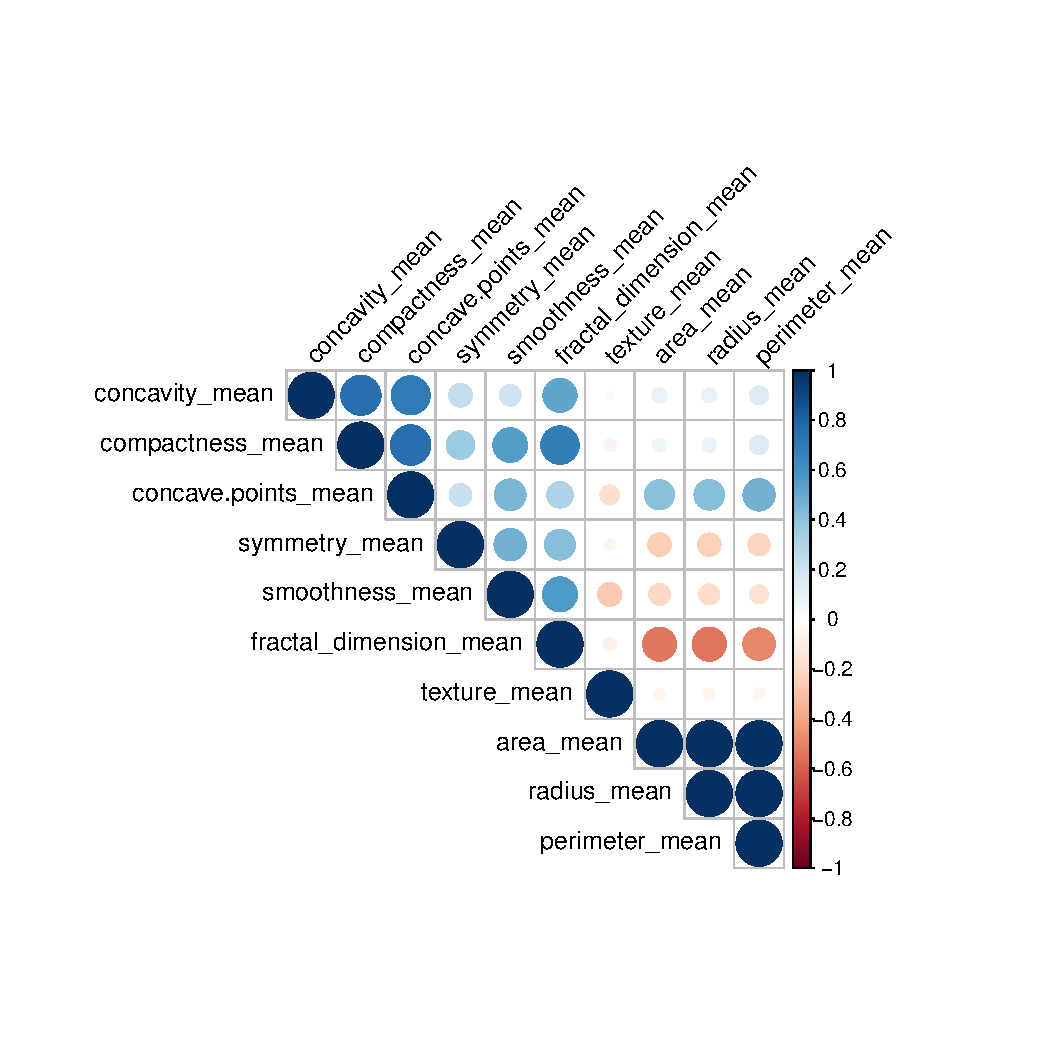
\includegraphics[width=.9\linewidth]{figs/q1_correlation_benign.pdf}
  \caption{Benign tumors}
\end{subfigure}
\caption{Correlation matrices}
\end{figure}

An even more visual way to assess the correlation between the class of the observation and the explanatory variables is a scatter where points are color coded respectively to their class :

\begin{figure}[H]
    \centering
    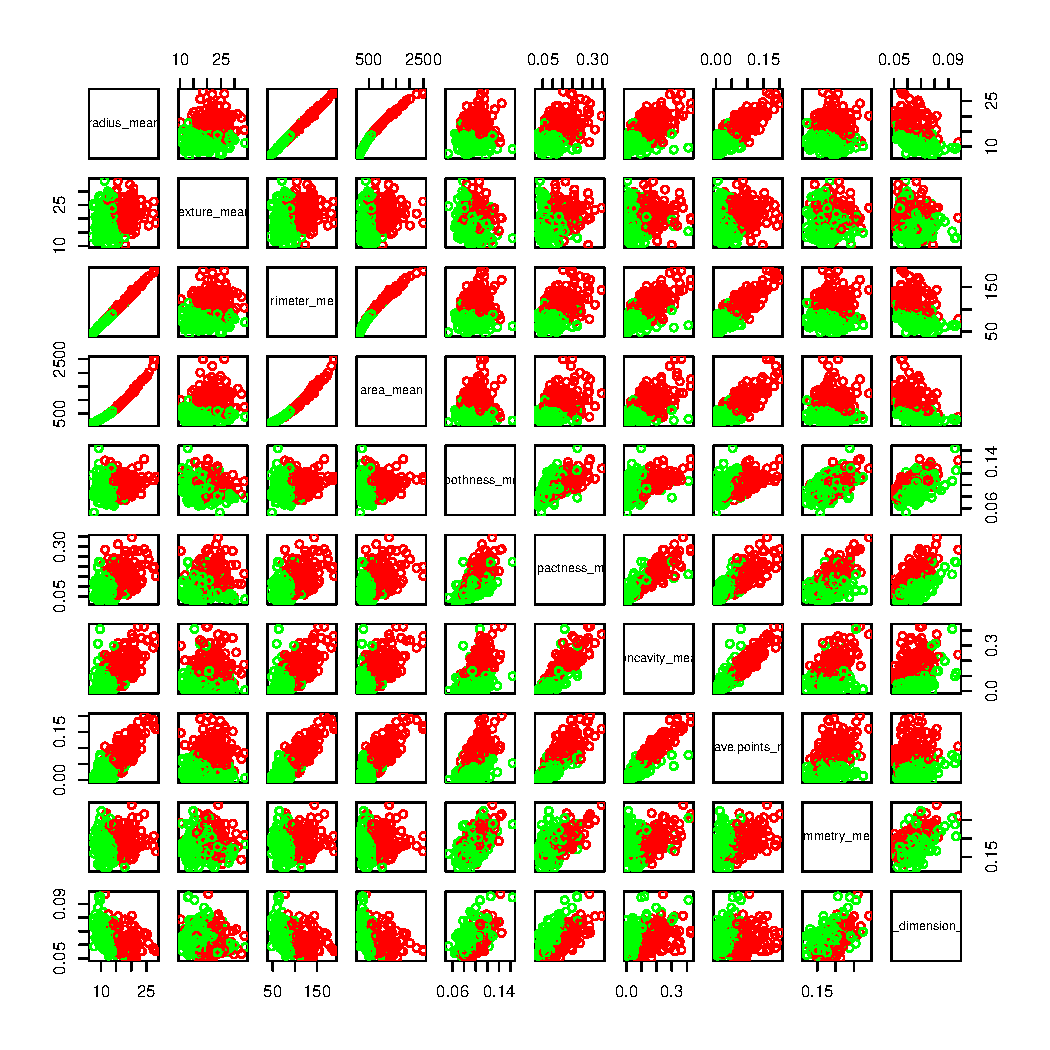
\includegraphics[width=.55\textwidth]{figs/q1_pairs.pdf}
    \caption{Caption}
    \label{fig:scatterplot}
\end{figure}

By looking at the figures here above, we again clearly see a correlation between the class of an observation and the explanatory variables values. Indeed, the values corresponding to benign tumors are concentrated to the left, representing smaller values. We can even see a clear linear correlation for the variables relative to the tumor's size. 


\subsection{Adequacy conclusion}
By exploring the data in these ways, we can gain a better understanding of whether the explanatory variables contain useful information for classifying observations into the two groups defined by the binary indicator and knowing the data has been collected on several period of times with a lot of observations, we can then clearly conclude that we can use our classification techniques on this dataset.